\chapter{에너지, 곡률, 복사}

\lectureoverview{뉴턴 역학 모형에서 두 가지 제약을 풀면 훨씬 더 많은 것을 알 수 있다. 첫째, 공변은하의 총에너지가 정확히 0일 필요는 없다. 에너지를 임의의 값으로 두면 일반상대성이론에서 공간 곡률로 재해석될 \(a^{-2}\) 항이 생긴다. 둘째, 우주의 원천이 압력이 없는 물질일 필요도 없다. 광자의 파장은 척도인자에 따라 늘어나므로 복사의 밀도는 \(a^{-4}\)에 따라 희석되고, 팽창 법칙은 \(a(t)\propto t^{1/2}\)가 된다. 따라서 물질과 복사가 함께 있는 우주는 작은 \(a\)에서 복사가 지배하고, 더 큰 \(a\)에서는 물질이 지배한다. 이 과정에서 국소적인 뉴턴 역학적 운동과 전역적인 상대론적 기하를 구분하고, 일반상대성이론 없이는 답할 수 없는 질문도 살펴본다.}

\section{뉴턴 역학으로 알 수 있는 것}

모형을 확장하기 전에 앞서 살펴본 뉴턴 역학 계산이 애초에 왜 성립했는지 물어보자. 실제 우주는 일반상대성이론으로 기술되며, 그 공간 기하는 전역적으로 유클리드 기하일 필요가 없다. 그렇지만 매끄러운 곡면 공간도 충분히 작은 근방에서는 거의 평평하다. 지구 표면의 작은 부분이 평면처럼 보이는 것과 마찬가지로, 곡률 반지름보다 훨씬 작은 우주 영역은 평평한 것으로 다룰 수 있다.

``작다''는 말은 곡률 척도에 비해 작다는 뜻이다. 그 영역의 크기는 여전히 수십억 광년일 수 있다. 그 안에서 은하들의 상대적 특이속도가 비상대론적이고 중력장이 약하다면, 이웃 은하들의 운동은 뉴턴 역학으로 다룰 수 있다. 따라서 뉴턴 역학 계산은 아인슈타인 이론과 경쟁하는 이론이 아니다. 그것은 더 완전한 기술의 국소적 저속도 극한이다.

여기서 곧바로 주의할 점이 있다. 복사는 느리게 움직이지 않는다. 광자와 상대론적 상태에 있는 중성미자는 보통의 뉴턴 역학적 입자 기체로 다룰 수 없다. 뉴턴 역학적 논리는 팽창 방정식을 정리하는 데 계속 유용하지만, 그 오른쪽의 원천은 정지질량 밀도에서 에너지 밀도로 확장되어야 한다. 바로 이 지점에서 근사의 한계가 드러나기 시작한다.

\section{척도인자 되짚어 보기}

은하가 균일하게 분포한다고 하고, 평균적인 우주 흐름을 따라 움직이는 격자에 좌표를 붙이자. 고정된 공변 좌표 \(x\)에 있는 은하의 물리적 거리는 선택한 원점으로부터
\begin{equation}
D(t)=a(t)x
\label{eq:c02-distance}
\end{equation}
이다. 척도인자 \(a(t)\)는 좌표상 간격을 물리적 간격으로 바꾸어 준다.

\(a\)의 절댓값은 관례에 따라 정한다. 모든 공변 좌표를 일정한 상수배로 재조정하면, 같은 물리적 거리를 \(a\)를 그 역수만큼 재조정해 나타낼 수 있다. 따라서 \(a\)와 좌표 셀 하나에 할당된 질량은 각각 따로 불변량이 아니다. 척도인자의 비와 분수 팽창률은 불변량이다.
\begin{equation}
\frac{a(t_2)}{a(t_1)},
\qquad
H(t)\equiv\frac{\dot a}{a}.
\label{eq:c02-hubble}
\end{equation}
실제로 고정된 상수 \(\alpha\)에 대해 \(a'=\alpha a\)라면, \(\dot a'/a'=\dot a/a\)이다.

\(\nu_m\)를 공변 좌표 부피 단위 하나에 들어 있는 질량이라고 하자. 격자의 좌표 표기를 바꾸면 그 수치는 달라지지만, 보통 물질이 보존되는 동안에는 시간에 따라 일정하다. 공변 단위 정육면체의 물리적 부피는 \(a^3\)이므로 물질 밀도는
\begin{equation}
\boxed{\rho_m(a)=\frac{\nu_m}{a^3}.}
\label{eq:c02-matter-density}
\end{equation}
이다. 이 \(a^{-3}\) 희석은 단순히 부피가 커지는 데 따른 것이다. 공변 상자 안의 정지에너지는 그대로인 채 부피만 커진다.

실제 은하들이 격자에 단단히 고정되어 있는 것은 아니다. 은하들은 은하군 안에서 공전하고, 은하단으로 낙하하며, 평균 흐름에 대한 작은 속도를 가진다. 척도인자는 큰 규모에서 평활화한 운동을 기술하며, 이와 같은 국소적 편차를 \emph{특이속도}라고 한다.

\begin{classroomqa}
\audiencequestion{모든 은하가 다른 모든 은하로부터 정확히 방사형으로 멀어져야 하나요?}
\lecturerresponse{평균화한 허블 흐름만 그런 형태를 띱니다. 은하의 실제 운동은 공통 팽창과 주변 구조 때문에 생기는 특이속도의 합입니다. 이는 소용돌이가 겹쳐 있는 강물의 흐름과 비슷합니다. 소용돌이는 국소적으로 영향을 주지만 큰 규모의 흐름을 없애지는 않습니다. \lecturetimestamp{00:24:47--00:26:33}}
\end{classroomqa}

뉴턴 역학적 총에너지가 영인 압력 없는 물질에 대해, 앞선 강의에서는 다음을 얻었다
\begin{equation}
H^2=\frac{8\pi G}{3}\rho_m
=\frac{8\pi G\nu_m}{3a^3}.
\label{eq:c02-zero-energy-friedmann}
\end{equation}
전체 격자의 정규화는 임의적이므로, 잠시 \(8\pi G\nu_m/3=1\)이 되도록 단위를 택할 수 있다. 팽창하는 해에서는
\begin{equation}
\frac{\dot a}{a}=\frac{1}{a^{3/2}},
\qquad
\dot a=\frac{1}{\sqrt a}.
\end{equation}
미분 관계를 역으로 풀어 적분하면 다음을 얻는다.
\begin{equation}
\frac{dt}{da}=\sqrt a,
\qquad
t-t_B=\frac{2}{3}a^{3/2},
\end{equation}
여기서 \(t_B\)은 이 이상화된 해가 \(a=0\)에 도달하는 시간이다. 따라서
\begin{equation}
\boxed{a(t)\propto (t-t_B)^{2/3}.}
\label{eq:c02-matter-law}
\end{equation}
물질만으로 이루어진 이 임계 모형에서 우주는 영원히 팽창한다. \(\dot a\propto a^{-1/2}\)이므로 팽창은 느려지지만, \(\dot a\)는 \(a\)의 어떤 유한한 값에서도 영이 되지 않는다.

\begin{figure}[ht]
\centering
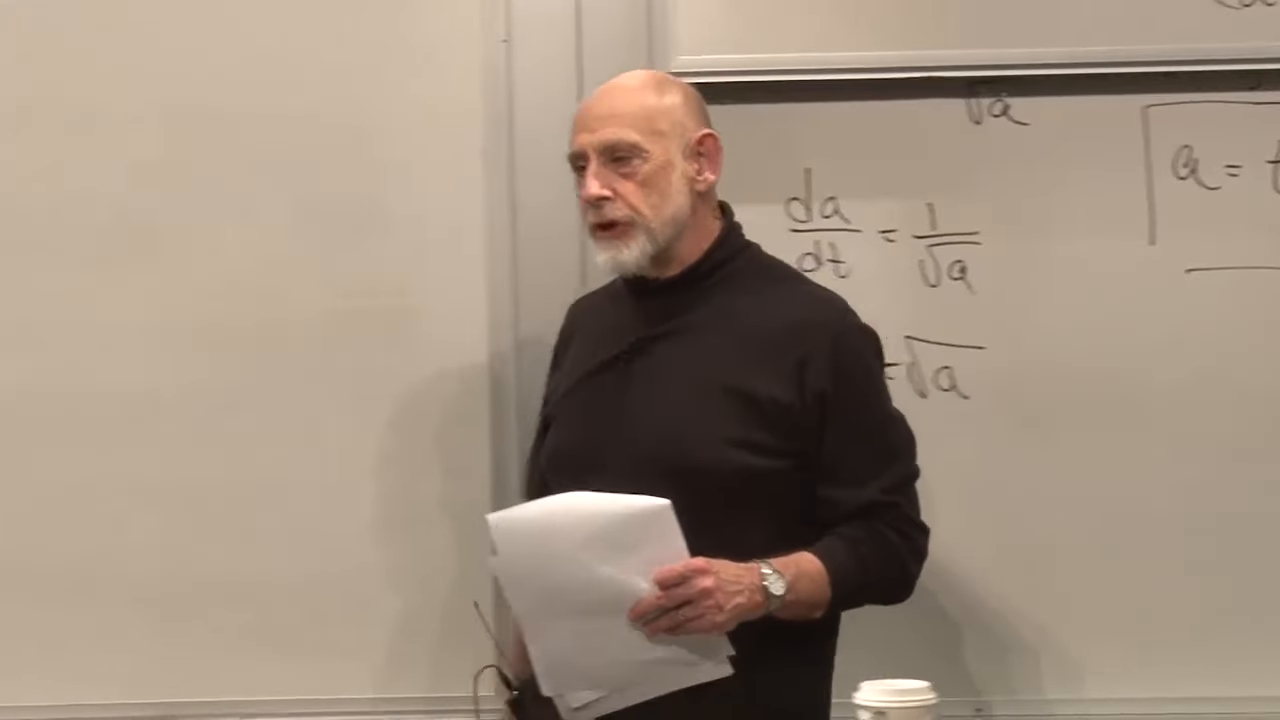
\includegraphics[width=0.68\textwidth]{lecture_02_figure_02.png}
\caption{복습 판서에는 \(\dot a=1/\sqrt a\)와 상자 안에 표시한 물질 지배 팽창 법칙 \(a\propto t^{2/3}\)가 적혀 있다. 중간 대수식은 일부 가려져 있어 식~\eqref{eq:c02-zero-energy-friedmann}--\eqref{eq:c02-matter-law}으로 보완했다.}
\label{fig:c02-matter-recap}
\lectureframe{00:29:20.838}
\end{figure}

\begin{classroomqa}
\audiencequestion{왜 음의 제곱근은 버렸나요?}
\lecturerresponse{방정식 자체가 음의 제곱근을 버린 것은 아니다. 식~\eqref{eq:c02-zero-energy-friedmann}은 \(H^2\)를 정할 뿐, \(H\)의 부호를 정하지 않는다. 양의 제곱근은 팽창을, 음의 제곱근은 수축을 나타낸다. 행성이 만드는 중력장 안의 바위는 같은 에너지 방정식을 따르면서도 바깥쪽이나 안쪽으로 움직일 수 있다. 초기 조건이 어느 해를 따를지 결정한다. 여기서 논의하는 우주가 팽창 중이므로 팽창하는 해를 선택했다. \lecturetimestamp{00:23:09--00:24:46}}
\end{classroomqa}

다음 모형에서도 암흑에너지는 다루지 않는다. 현재의 가속 팽창을 지배하는 성분을 더하기 전에, 먼저 오래된 물질·복사 모형을 이해하려는 의도적인 선택이다. 반면 암흑물질은 이미 물질 항에 포함되어 있다. 비상대론적 암흑물질도 \(a^{-3}\)에 따라 희석되기 때문이다.

\begin{classroomqa}
\audiencequestion{오늘날에는 암흑에너지가 지배 성분 아닌가요?}
\lecturerresponse{그렇다. 여기서 전개하는 두 성분 모형은 현재의 가속 팽창이 발견되기 전에 표준적으로 가르치던 우주론이다. 암흑물질은 물질에 포함되고, 암흑에너지는 별도로 도입할 세 번째 성분이다. 오래된 모형에서 출발하면 각각의 항을 더할 때 무엇이 달라지는지 알 수 있다. \lecturetimestamp{00:28:02--00:28:45}}
\end{classroomqa}

\section{에너지 상수 다시 도입하기}

에너지를 0으로 두는 것은 특별한 초기 조건이다. 이를 풀기 위해 균일한 구의 경계에 있는 질량 \(m\)인 은하를 다시 생각하자. 그 은하의 공변 반지름을 \(x\)라고 두면,
\begin{equation}
D=ax,
\qquad
\dot D=\dot a x.
\label{eq:c02-comoving-particle}
\end{equation}
뉴턴의 껍질 정리에 따르면 구 안쪽의 질량 \(M(D)\)만 반지름 방향 가속도에 영향을 주며, 바깥쪽 구형 껍질은 알짜 힘을 가하지 않는다. 은하의 보존되는 뉴턴 역학적 에너지는
\begin{equation}
\frac{1}{2}m\dot D^{\,2}-\frac{GM(D)m}{D}=E.
\label{eq:c02-newton-energy}
\end{equation}
이다. 두 항에 모두 인자 \(m\)가 들어간다. 판서할 때 빠뜨리기 쉽지만, 이를 남겨 두면 마지막 상수가 시험 질량 단위당 에너지라는 점이 분명해진다.

균일성에 따라 대표 은하를 \(x=1\)에 둬도 된다. 그러면 \(D=a\), \(\dot D=\dot a\)이고, 구의 부피와 질량은
\begin{equation}
V_{\rm sph}=\frac{4\pi}{3}a^3,
\qquad
M(a)=\rho_m V_{\rm sph}=\frac{4\pi}{3}\rho_m a^3.
\label{eq:c02-enclosed-mass}
\end{equation}
이다. 판서에서는 부피를 나타낼 때와 옆에 반지름 속도를 적을 때 모두 \(V\)를 쓴다. 혼동을 피하기 위해 여기서는 명확한 기호 \(V_{\rm sph}\)와 \(\dot D\)를 사용한다.

\begin{figure}[ht]
\centering
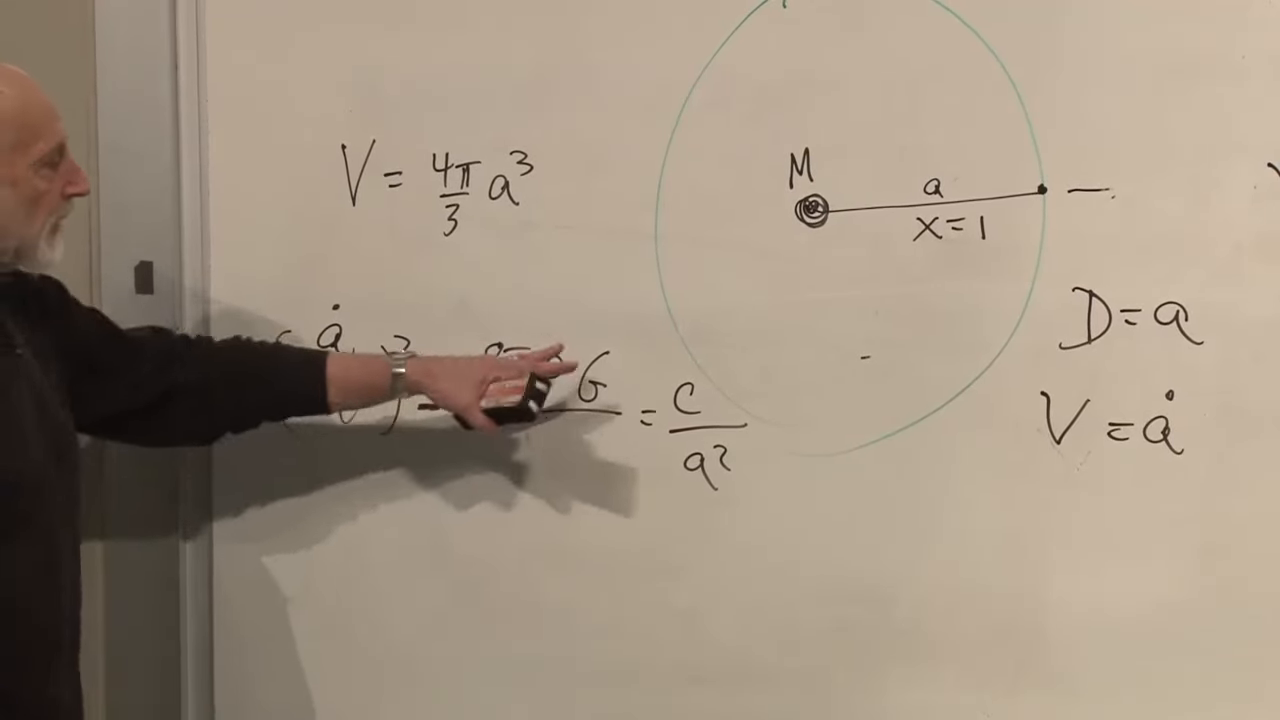
\includegraphics[width=0.86\textwidth]{lecture_02_figure_03.png}
\caption{구 안에 포함된 질량과 에너지가 0이 아닌 경우의 프리드만 방정식. 보이는 표기에는 \(V_{\rm sph}=4\pi a^3/3\), 중심 질량 \(M\), \(x=1\), \(D=a\), \(\dot D=\dot a\)가 포함되어 있다. 방정식 일부는 강사에 가려져 있어 아래에서 대수적으로 복원한다.}
\label{fig:c02-energy-board}
\lectureframe{00:37:59.876}
\end{figure}

\begin{figure}[ht]
\centering
\begin{tikzpicture}[scale=1.05,>=Latex]
  \draw[thick] (0,0) circle (2.6);
  \fill (0,0) circle (2.2pt) node[below left=2pt] {\(M(a)\)};
  \draw[thick,->] (0,0) -- (2.58,0);
  \fill (2.6,0) circle (2.2pt) node[right=4pt] {galaxy \(m\)};
  \node[above] at (1.30,0.04) {\(D=ax\)};
  \node[below] at (1.30,-0.04) {\(x=1\Rightarrow D=a\)};
  \draw[->,blue!60!black,thick] (2.63,0.18) -- (3.55,0.72)
    node[right] {\(\dot D=\dot a\)};
  \node at (0,-3.05) {\(M(a)=\frac{4\pi}{3}\rho_m a^3\)};
\end{tikzpicture}
\caption{\(x=1\)에서의 뉴턴 역학적 구를 깔끔하게 다시 그린 그림. 바깥쪽 껍질들의 힘은 상쇄되므로 경계의 은하는 구 안에 포함된 질량에만 반응한다.}
\label{fig:c02-sphere-redraw}
\end{figure}

\(D=a\)를 식~\eqref{eq:c02-newton-energy}에 대입하고 \(m/2\)로 나눈 다음, 상수를
\begin{equation}
C\equiv\frac{2E}{m}.
\end{equation}
로 정의하자. 그러면
\begin{equation}
\dot a^{\,2}-\frac{2GM(a)}{a}=C.
\label{eq:c02-energy-a}
\end{equation}
를 얻는다. 이를 \(a^2\)로 나누고 식~\eqref{eq:c02-enclosed-mass}을 이용하면
\begin{equation}
\left(\frac{\dot a}{a}\right)^2-
\frac{8\pi G}{3}\rho_m=\frac{C}{a^2},
\label{eq:c02-energy-form}
\end{equation}
또는 동등하게
\begin{equation}
\boxed{H^2=\frac{8\pi G}{3}\rho_m+\frac{C}{a^2}.}
\label{eq:c02-friedmann-C}
\end{equation}
가 된다. 이는 압력이 없는 물질에 대한 첫 번째 프리드만 방정식을 뉴턴 역학의 에너지 관례로 쓴 것이다. 새로 나타난 \(a^{-2}\) 항은 대표 은하가 탈출 에너지보다 큰 에너지로, 그 에너지로, 또는 더 낮은 에너지로 출발했는지를 반영한다.

\(\rho_m=\nu_m/a^3\)를 대입하고 다음과 같이 정의하면 편리하다.
\begin{equation}
A_m\equiv\frac{8\pi G\nu_m}{3}>0,
\end{equation}
그러면
\begin{equation}
H^2=\frac{A_m}{a^3}+\frac{C}{a^2},
\qquad
\dot a^{\,2}=\frac{A_m}{a}+C.
\label{eq:c02-energy-branches}
\end{equation}
가 된다. 이 방정식은 곧바로 적분하기보다 극한별로 읽을 때 더 많은 정보를 준다.

\subsection{양의 에너지}

\(C>0\)이면 작은 \(a\)에서 물질 항 \(A_m/a^3\)이 지배적이다. 따라서 초기 팽창은 물질 우주에서의 법칙 \(a\propto t^{2/3}\)을 따른다. 그러나 큰 \(a\)에서는 \(H^2\)에서 \(C/a^2\) 항이 지배적이며, 이는 다음 식과 같다.
\begin{equation}
\dot a^{\,2}\longrightarrow C.
\end{equation}
팽창 속도는 일정한 값에 가까워진다.
\begin{equation}
a(t)\sim\sqrt C\,t.
\label{eq:c02-positive-late}
\end{equation}
이는 탈출 속도보다 빠르게 사과를 던지는 상황에 대응하는 우주론적 사례다. 중력은 사과의 속도를 계속 줄이지만, 아주 멀리 가면 사과는 영이 아닌 점근 속도를 유지한다.

\subsection{에너지 0}

\(C=0\)일 때 식~\eqref{eq:c02-energy-branches}은 임계 해 \(a\propto t^{2/3}\)를 되돌려 준다. \(\dot a\)는 0에 가까워지지만, 우주는 끝없이 팽창한다. 이는 정확히 탈출 에너지에 해당하는 경우다.

\subsection{음의 에너지}

\(C=-|C|<0\)이면
\begin{equation}
H^2=\frac{A_m}{a^3}-\frac{|C|}{a^2}
=\frac{A_m-|C|a}{a^3}.
\label{eq:c02-negative-energy}
\end{equation}
이다. 척도인자는 다음 값을 넘을 수 없다.
\begin{equation}
a_{\max}=\frac{A_m}{|C|},
\label{eq:c02-amax}
\end{equation}
그 지점에서 우변이 0이 되기 때문이다. 팽창하는 해는 \(a_{\max}\)에 도달할 때 \(\dot a=0\)이 된다. 이후에는 수축하는 해를 따른다. 뉴턴 역학의 그림으로 보면 탈출 속도보다 느리게 던진 사과처럼 올라갔다가 방향을 바꾸어 떨어진다.

\begin{classroomqa}\audiencequestion{우변이 \(H^2\)와 같아 음수가 될 수 없는데, 모형은 어떻게 다시 수축할 수 있습니까?}\lecturerresponse{우변은 결코 음수가 되지 않는다. 팽창하는 동안 우변은 \(a_{\max}\)에서 영으로 감소한다. 그 지점에서 \(H=0\)이다. 그러면 해는 양의 제곱근에서 음의 제곱근으로 바뀌고, \(\dot a<0\)인 채 허용된 영역을 되짚는다. 식이 영을 지나 계속 이어질 수 있다고 생각하기 쉽지만, 이는 잘못이다. 영은 실수 \(H\)가 이어질 수 있는 경계이지, 그 너머로 계속 이어질 수 있는 값이 아니다. \lecturetimestamp{00:48:43--00:53:03}}\end{classroomqa}

따라서 뉴턴 역학의 세 가지 에너지 값은 세 가지 정성적 역사를 낳는다. \(C<0\)이면 재붕괴하고, \(C=0\)이면 임계적으로 탈출하며, \(C>0\)이면 \(\dot a\)가 점근적으로 일정한 채 영원히 팽창한다. 놀랍게도 일반상대성이론은 다음 단계에서 이 같은 경우들에 기하학적 의미를 부여한다.

\section{에너지에서 곡률로}

식~\eqref{eq:c02-friedmann-C}의 에너지 항을 기하학 쪽으로 옮기고 다음과 같이 정의하자.
\begin{equation}
k\equiv-C.
\label{eq:c02-k-definition}
\end{equation}
그러면
\begin{equation}
\boxed{H^2+\frac{k}{a^2}=\frac{8\pi G}{3}\rho.}
\label{eq:c02-friedmann-k}
\end{equation}
이다. 판서에서는 \(C\), \(K\), \(\kappa\)를 번갈아 사용하며, 항을 등식의 반대편으로 옮길 때 부호가 하나 흡수된다. 식~\eqref{eq:c02-k-definition}에 따라 여기서의 부호 관례가 정해진다. 뉴턴 역학적 에너지가 양수이면 \(k<0\), 에너지가 0이면 \(k=0\), 음수이면 \(k>0\)이다.

\begin{figure}[ht]
\centering
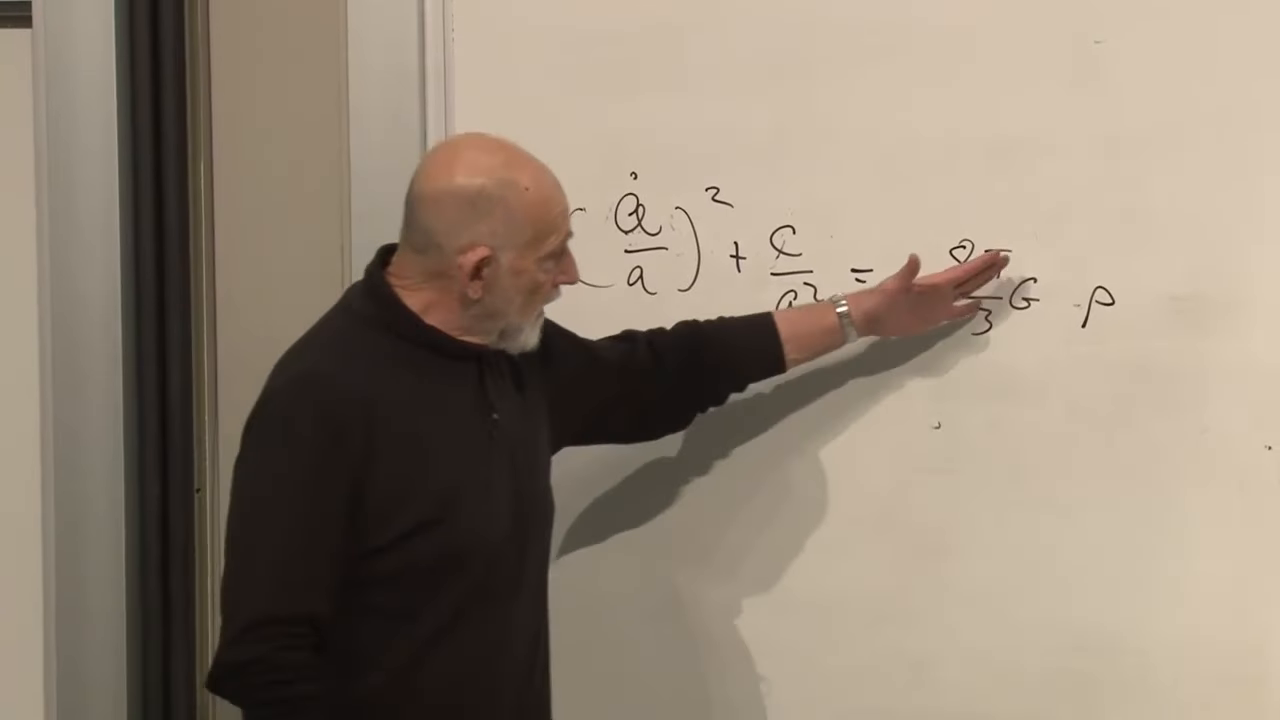
\includegraphics[width=0.76\textwidth]{lecture_02_figure_04.png}
왼쪽에는 기하를, 오른쪽에는 원천을 둔 프리드만 방정식. 이 화면은 개념적인 구분을 보여 주며, 아인슈타인의 텐서 방정식 전체를 나타내지는 않는다.\caption{
}
\label{fig:c02-geometry-source}
\lectureframe{00:55:22.810}
\end{figure}

이런 배열은 아인슈타인 방정식을 축약해 보여 준다. 왼쪽은 \(H\)를 통한 팽창과 \(k/a^2\)를 통한 공간 곡률, 즉 기하를 나타낸다. 오른쪽은 물질 원천을 나타낸다. 뉴턴 역학에서 원천은 질량 밀도였다. 상대론에서는 이를 에너지와 운동량으로 나타내며, 완전한 기술에는 응력-에너지 텐서를 쓴다. 균일하고 등방적인 우주에서 첫 번째 프리드만 방정식은 전체 에너지 밀도 \(\rho\)에 의존한다.

보통의 단위를 유지하면 질량 밀도는 정지에너지 \(\rho_{\rm mass}c^2\)를 통해 기여한다. 이제부터는 \(c=1\)로 두어 질량과 에너지를 같은 단위로 쓴다. 그러면 기호 \(\rho\)에는 정지질량, 운동에너지, 복사 및 그 밖의 균일한 에너지 성분이 포함될 수 있다.

\begin{figure}[ht]\centering
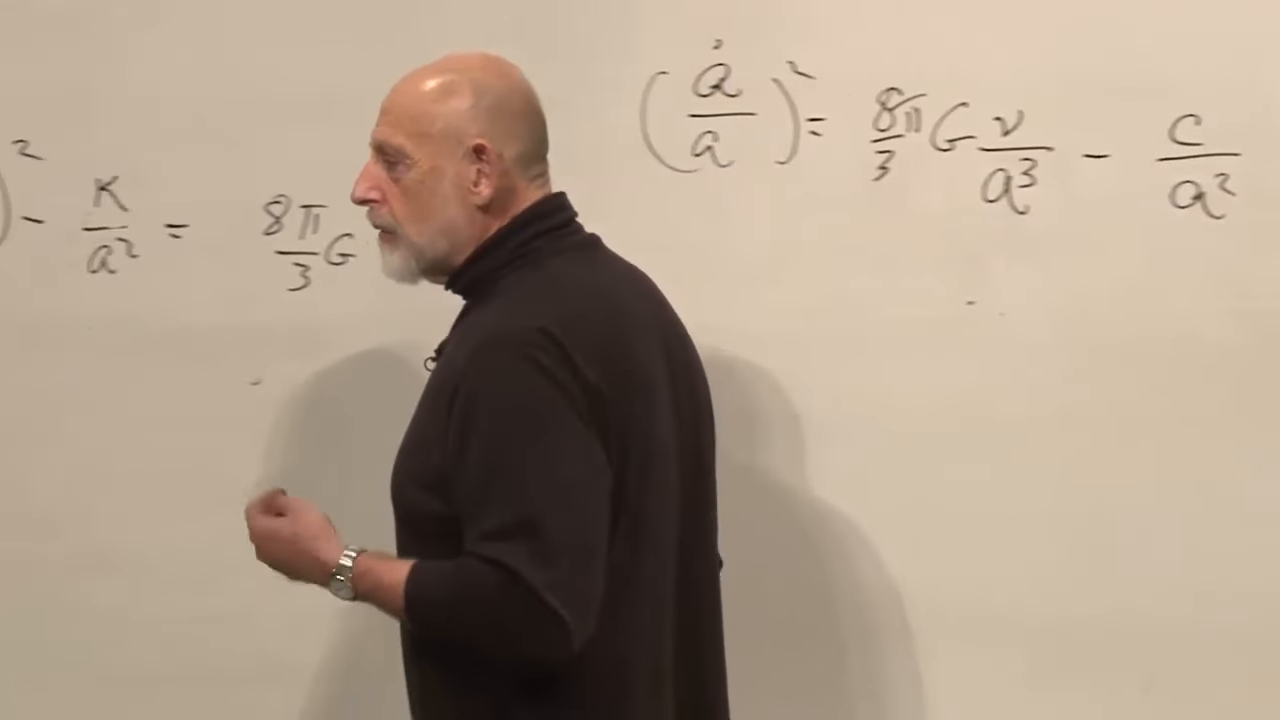
\includegraphics[width=0.88\textwidth]{lecture_02_figure_05.png}\caption{프리드먼 방정식을 칠판에 나란히 적은 두 형태: \(\rho\)를 사용하는 곡률 형태와 \(\rho_m=\nu_m/a^3\)을 대입한 뒤 얻는 물질 형태. 칠판의 표기는 바뀌지만, ~\eqref{eq:c02-k-definition}은 여기서 부호 규약을 고정해 둔다.}\label{fig:c02-curvature-comparison}\lectureframe{00:57:52.659}\end{figure}

기하학적 해석은 전역적인 것이다. 상대론적 모형에서 \(k=0\)는 평평한 공간 단면을, \(k>0\)는 양의 곡률을 가진 구면 단면을, \(k<0\)는 음의 곡률을 가진 쌍곡 단면을 나타낸다. 뉴턴 역학적 유도에서는 이런 전역 기하학을 갖추지 않고도 같은 진화 방정식을 얻었다. 따라서 영이 아닌 에너지 상수는 곡률을 놀라울 만큼 정확하게 모방하지만, 그 자체로 곡률을 지닌 공간을 유도한 것은 아니다.

\begin{classroomqa}
\audiencequestion{기하가 다른데도 뉴턴 역학과 일반상대성이론에서 같은 팽창 방정식이 나올 수 있는 이유는 무엇인가요?}
\lecturerresponse{일반상대성이론에는 평탄한 경우도 포함되며, 매끄러운 기하는 국소적으로 언제나 거의 평탄하다. 더 놀라운 점은 뉴턴 역학의 에너지 상수가 상대론적 공간 곡률이 차지하는 자리와 정확히 같은 곳에 진화 방정식에 들어간다는 것이다. 동역학적 공식은 일치하지만 전역적 해석은 다르다. 유클리드 뉴턴 공간이 몰래 구면 공간이나 쌍곡 공간으로 변한 것은 아니다. 세 가지 기하는 일반상대성이론 안에서 구성해야 한다. \lecturetimestamp{01:20:59--01:24:20}}
\end{classroomqa}

\section{팽창하는 상자 안의 복사}

이제 우주의 구성 성분을 바꾸어 보자. 공변 단위 정육면체 하나를 생각하자. 그 물리적 부피는 \(a^3\)이다. 비상대론적 물질의 경우 상자 안의 입자 수는 일정하고 각 입자의 정지에너지도 거의 일정하므로 \(\rho_m\propto a^{-3}\)가 된다. 복사에는 추가 효과가 있다. 우주가 팽창하면 광자마다 에너지가 줄어든다.

파장이 \(\lambda\)인 광자의 에너지는
\begin{equation}
E_\gamma=\frac{hc}{\lambda},
\qquad
E_\gamma\propto\lambda^{-1}.
\label{eq:c02-photon-energy}
\end{equation}
이다. 균일한 팽창에서는 자유롭게 전파되는 파장이 척도인자에 따라 늘어난다.
\begin{equation}
\frac{\lambda(t_2)}{\lambda(t_1)}
=\frac{a(t_2)}{a(t_1)},
\qquad
\lambda\propto a.
\label{eq:c02-redshift}
\end{equation}
이것이 우주론적 적색편이다. 따라서
\begin{equation}
E_\gamma\propto a^{-1}.
\label{eq:c02-photon-redshift}
\end{equation}
이다. 공변 상자 안의 광자 수가 보존되면 전체 복사 에너지는 \(a^{-1}\)에 따라 감소한다. 이를 물리적 부피 \(a^3\)로 나누면
\begin{equation}
\boxed{\rho_r(a)=\frac{\nu_r}{a^4}.}
\label{eq:c02-radiation-density}
\end{equation}
를 얻는다. 여기서 \(\nu_r\)는 자유롭게 전파되는 복사 밀도의 일정한 크기 계수다. 복사 밀도에는 물질보다 \(a\)의 역수가 한 번 더 들어간다. 세 제곱은 공간적 희석에서, 나머지 한 제곱은 모든 광자의 적색편이에서 온다.

기타 줄의 비유는 유용한 직관을 준다. 줄에 맞춰진 정상 모드에는 반파장이 정수 개 들어간다. 줄을 천천히 늘이면 그 정수는 연속적으로 바뀔 수 없으므로, 파장이 새 길이에 맞춰 조정된다. 마찬가지로 천천히 팽창하는 고리 위의 파동에서는 마디 수가 단열 불변량이므로 파장이 고리의 둘레를 따른다. 일반적인 파동은 이런 모드들의 합으로 분해할 수 있다.

이 비유가 팽창하는 시공간에서 맥스웰 방정식을 푸는 일을 대신하지는 않는다. 이는 식~\eqref{eq:c02-redshift}의 통제된 직관이다. 즉, 기하가 천천히 팽창하면 모드 표지는 보존되고 물리적 파장은 변한다.

\begin{classroomqa}
\audiencequestion{이 논증에 전도성 벽이나 반사벽이 꼭 필요한가요? 물리적인 벽이 없는 빈 팽창 공간에서는 어떻게 되나요?}
\lecturerresponse{벽은 계산을 정리하기 위한 도구이지, 우주가 도체로 둘러싸여 있다는 뜻이 아니다. 완전한 증명은 팽창하는 계량에서 파동 전파를 다루어 얻는다. 여기서는 자유롭게 전파되는 파장의 크기가 \(a\)에 비례한다는, 관측으로 확인되고 상대론적으로 유도된 사실을 이용한다. 상자는 광자와 물리적 부피를 세는 데 도움이 될 뿐, 우주론적 적색편이를 일으키지는 않는다. \lecturetimestamp{01:02:21--01:04:37}}
\end{classroomqa}

\begin{classroomqa}
\audiencequestion{파장이 왜 물리적 길이를 고정해서 유지하지 않고 격자를 따라 변해야 하나요?}
\lecturerresponse{둘레가 단열적으로 변하는 고리의 모드를 생각해 보자. 정수인 마디 수는 연속적으로 변할 수 없으므로 허용되는 파장은 고리의 크기에 따라 변해야 한다. 일반적인 파동을 푸리에 모드로 전개해도 모드마다 같은 결론을 얻는다. 이것이 필요한 단열적 직관이다. 정확한 진술은 곡률 시공간의 장 이론에서 다룬다. \lecturetimestamp{01:34:18--01:38:33}}
\end{classroomqa}

\subsection{복사 지배 해}

일단 곡률을 무시하고 식~\eqref{eq:c02-radiation-density}를 프리드만 방정식에 대입하면
\begin{equation}
H^2=\frac{8\pi G\nu_r}{3a^4}
\equiv\frac{A_r}{a^4},
\qquad A_r>0.
\label{eq:c02-radiation-friedmann}
\end{equation}
를 얻는다. 팽창하는 해에서는
\begin{equation}
\frac{\dot a}{a}=\frac{\sqrt{A_r}}{a^2},
\qquad
\dot a=\frac{\sqrt{A_r}}{a}.
\end{equation}
이므로
\begin{equation}
a\,da=\sqrt{A_r}\,dt,
\qquad
\frac{a^2}{2}=\sqrt{A_r}(t-t_B),
\end{equation}
이고,
\begin{equation}
\boxed{a(t)\propto(t-t_B)^{1/2}.}
\label{eq:c02-radiation-law}
\end{equation}
이다. 지수 \(1/2\)과 \(2/3\)의 차이는 눈으로 보기에는 작아도 물리적으로는 결정적이다. 초기 우주의 팽창률, 온도, 반응 동결 시점과 지평선 크기는 모두 어느 성분이 지배하는지에 달려 있다.

\section{물질과 복사가 함께 있는 우주}

서로 따로 보존되는 물질과 복사의 밀도는 더해진다.
\begin{equation}
\rho(a)=\rho_m(a)+\rho_r(a).
\end{equation}
이 둘을 비교하는 동안 곡률을 무시하면
\begin{equation}
\boxed{H^2=\frac{C_m}{a^3}+\frac{C_r}{a^4},}
\label{eq:c02-mixed-friedmann}
\end{equation}
를 얻는다. 여기서 \(C_m,C_r>0\)이다. 판서에서는 두 계수를 먼저 \(C_1\)와 \(C\)로 표시했다가, 두 번째 기호가 다른 상수를 뜻하도록 말로 정정한다. 식~\eqref{eq:c02-mixed-friedmann}에는 그 정정이 명시되어 있다.

\begin{figure}[ht]\centering
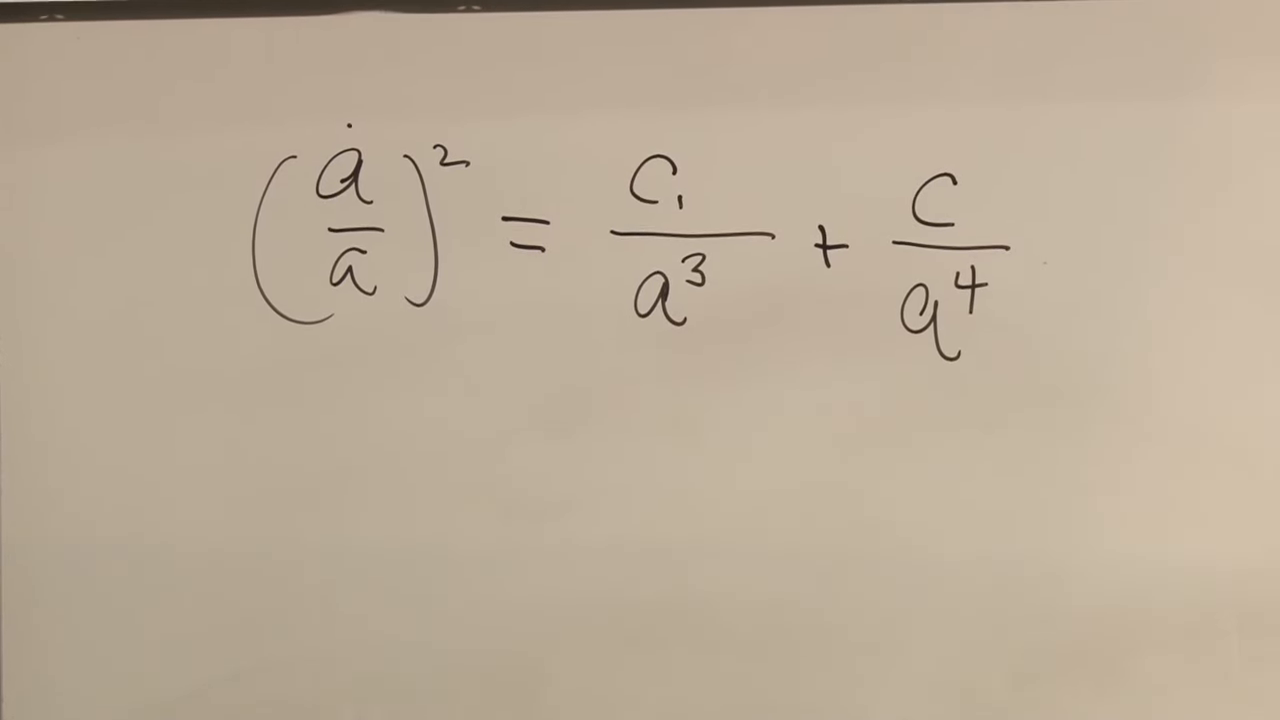
\includegraphics[width=0.74\textwidth]{lecture_02_figure_06.png}\caption{칠판에 적힌 물질과 복사가 함께 있는 방정식. 처음 적힌 두 번째 계수는 뒤이어 복사에만 해당하는 상수로 수정되며, 방정식 ~\eqref{eq:c02-mixed-friedmann}에서는 \(C_r\)로 표기한다.}\label{fig:c02-mixed-board}\lectureframe{01:11:37.997}\end{figure}

작은 \(a\)에서는 \(a^{-4}\)가 \(a^{-3}\)보다 더 빠르게 커지므로 복사 항이 우세하다.
\begin{equation}
a\ll a_{\rm eq}
\quad\Longrightarrow\quad
H^2\simeq\frac{C_r}{a^4},
\qquad
a(t)\propto t^{1/2}.
\end{equation}
더 큰 \(a\)에서는 물질 항이 우세하다.
\begin{equation}
a\gg a_{\rm eq}
\quad\Longrightarrow\quad
H^2\simeq\frac{C_m}{a^3},
\qquad
a(t)\propto t^{2/3}.
\end{equation}
두 항을 같게 놓으면 등가 척도를 바로 구할 수 있다.
\begin{equation}
a_{\rm eq}=\frac{C_r}{C_m}.
\label{eq:c02-equality-scale}
\end{equation}
이 등가는 광자 분리와 같은 사건이 아니다. 등가는 두 에너지 밀도가 같아지는 시점이고, 분리는 상호작용이 물질과 복사를 열적 접촉 상태로 유지하지 못하게 되는 시점이다.

복사 부문에는 광자와 초상대론적으로 움직이는 모든 종이 포함된다. 질량이 매우 작은 중성미자는 충분히 높은 온도에서 이렇게 거동하며, 중력자 배경도 같은 방식으로 스케일링된다. 질량이 있는 종이 비상대론적 상태가 되면 지배적인 정지질량 기여분이 물질처럼 스케일링되기 시작한다. 차가운 암흑물질은 복사 항이 아니라 \(C_m/a^3\)에 속한다.

\begin{classroomqa}
\classquestion{식~\eqref{eq:c02-mixed-friedmann}에서 어느 항이 먼저 지배하고, 나중에는 어느 항이 지배하나요?}
\lecturerresponse{작은 \(a\)에서는 \(a^{-4}\)가 \(a^{-3}\)보다 빠르게 커지므로 복사가 초기 팽창을 지배하고 \(a\propto t^{1/2}\)를 준다. \(a\)가 커지면 복사 대 물질 비율은 \(1/a\)에 따라 감소한다. 그러면 물질이 팽창을 지배하며 \(a\propto t^{2/3}\)를 준다. \lecturetimestamp{01:11:46--01:13:38}}
\end{classroomqa}

\begin{classroomqa}
\audiencequestion{물질과 복사의 상대적 양이 일정하다고 가정하나요?}
\lecturerresponse{밀도는 일정하지 않지만 성분들 사이의 에너지 교환이 효율적으로 일어나지 않게 되고 입자 생성이나 소멸을 무시할 수 있게 되면 계수 \(C_m\)와 \(C_r\)를 상수로 다룰 수 있다. 그러면 물질은 보존되는 공변 정지질량을, 자유 복사는 보존되는 공변 광자 수를 가진다. 적색편이가 복사에 추가로 \(a^{-1}\) 인자를 준다. 상호작용이 강하거나 입자가 소멸하는 시기에는 계산을 더 정교하게 해야 한다. \lecturetimestamp{01:13:39--01:14:53}}
\end{classroomqa}

\begin{classroomqa}
\audiencequestion{물질과 복사는 언제 강하게 상호작용하기를 멈췄나요?}
\lecturerresponse{대략적인 크기 추정으로는 광자가 보통 물질에서 분리된 시점이 \(10^5\)년이다. 정확한 재결합 역사는 뒤에서 계산하며, 물질--복사 등가와 혼동해서는 안 된다. 여기서 필요한 요점은 분리 이후 두 성분을 대략 서로 독립적으로 추적할 수 있다는 것이다. \lecturetimestamp{01:27:29--01:27:46}}
\end{classroomqa}

\begin{classroomqa}
\audiencequestion{팽창을 추적할 은하가 생기기 전인 초기 우주에 \(a\propto t^{1/2}\) 시대가 있었다는 것을 어떻게 알 수 있나요?}
\lecturerresponse{우리는 우주의 팽창 역사가 남긴 물리적 기록을 통해 이를 추론한다. 원시 핵합성은 반응률과 \(H(t)\) 사이의 초기 경쟁에 좌우된다. 우주 마이크로파 배경은 그보다 뒤의 열적 상태와 섭동을 기록한다. 은하 관측으로는 물질 시대의 거동을 더 직접적으로 확인할 수 있지만, 복사 시대는 이런 초기 우주 증거를 바탕으로 재구성한다. \lecturetimestamp{01:27:46--01:30:10}}
\end{classroomqa}

물질과 복사만 있는 모형은 의도적으로 불완전하다. 우주가 복사 지배에서 물질 지배로 넘어가는 고전적인 틀이다. 현재의 가속 팽창을 설명하려면 암흑에너지라는 별도의 원천이 필요하며, 이는 질적으로 다른 항을 더한다.

\section{적색편이된 에너지는 어디로 가는가}

\(E_\gamma\propto a^{-1}\)의 감소는 피할 수 없는 질문을 던진다. 광자의 에너지는 어디로 간 것일까? 반사벽이 있는 실제 팽창 상자에서는 복사가 압력을 가해 벽에 일을 한다. 열역학적으로는
\begin{equation}
dE=-p\,dV.
\label{eq:c02-pdv}
\end{equation}
이다. \(V\)가 커지면 복사 에너지는 줄어든다. 사라진 에너지는 벽을 움직이는 대상의 운동에너지, 변형 에너지 또는 열로 나타날 수 있다.

공변 상자에는 물질로 된 벽이 없다. 평균 팽창을 따라 움직이는 가상의 경계다. 광자는 그 경계를 통과하지만, 균일한 복사 열탕에서는 통계적으로 들어오는 흐름과 나가는 흐름이 균형을 이룬다. 상자는 용기가 아니지만 계산을 정리하는 부피로는 여전히 유효하다. 압력에 따른 일의 법칙은 공변 부피 안의 에너지가 어떻게 변하는지 여전히 기술한다.

복사에서는 \(p=\rho/3\)이고 \(E=\rho V\)이다. 그러므로 식~\eqref{eq:c02-pdv}에서
\begin{align}
d(\rho V)&=-\frac{\rho}{3}\,dV,\\
V\,d\rho&=-\frac{4}{3}\rho\,dV,\\
\frac{d\rho}{\rho}&=-\frac{4}{3}\frac{dV}{V}.
\end{align}
를 얻는다. \(V\propto a^3\)이므로 적분하면 \(\rho\propto a^{-4}\)가 되어 파장 논증과 일치한다. 이 열역학적 유도는 입자 수 밀도만이 아니라 각 광자의 에너지도 감소한다는 점을 분명히 보여 준다.

\begin{classroomqa}
\audiencequestion{적색편이된 광자의 에너지는 어디로 가나요? 우주 전체 에너지는 보존되나요?}
\lecturerresponse{물리적 벽이 있다면 복사가 벽에 일을 하므로 에너지 이동을 보통의 역학적 장부 정리로 설명할 수 있다. 우주 전체에 대해서는 문제가 더 미묘하다. 전역적 에너지 보존은 보통 시간 병진 대칭에서 나오지만, 팽창하는 시공간은 일반적으로 시간 병진 대칭이 아니며 유일하게 보존되는 총에너지를 가질 필요도 없다. 팽창 에너지를 이용한 유용한 뉴턴 역학적 비유를 만들 수는 있지만, 전역적인 결론을 확정하려면 일반상대성이론이 필요하다. 여기서는 두 기술 모두 유용하지만, 뉴턴 역학 모형만으로 전역적인 최종 결론을 내릴 수는 없다. \lecturetimestamp{01:16:51--01:20:58}}
\end{classroomqa}

\begin{classroomqa}
\audiencequestion{공변 상자는 가상이고 광자가 경계를 통과하는데도 압력에 따른 일을 유용한 그림으로 쓸 수 있는 이유는 무엇인가요?}
\lecturerresponse{균일성이 빠진 계산을 보완한다. 한 공변 부피에서 나가는 광자 하나마다 이웃 부피에서 들어오는 광자 하나가 통계적으로 평균적으로 대응한다. 국소적인 흐름은 평균적으로 상쇄되지만 물리적 부피와 파장은 변한다. 반사벽이 있는 상자는 일의 메커니즘을 구체적으로 보여 주고, 공변 상자는 실제 벽 없이도 같은 평균 보존 법칙을 나타낸다. \lecturetimestamp{01:24:22--01:27:28}}
\end{classroomqa}

\begin{classroomqa}
\audiencequestion{팽창은 광자 밀도만 낮추나요, 아니면 광자 하나하나의 에너지도 줄이나요?}
\lecturerresponse{둘 다 일어난다. 물리적 부피당 광자 수는 \(a^{-3}\)에 따라 줄고, 우주론적 적색편이는 광자 하나하나의 에너지를 추가로 \(a^{-1}\)만큼 낮춘다. 이는 복사에 대한 단열 냉각에 해당한다. 보통 기체도 천천히 팽창하며 일을 하는 동안 냉각되지만, 급격한 자유 팽창은 열역학적으로 다른 과정이다. \lecturetimestamp{01:42:30--01:45:55}}
\end{classroomqa}

\section{후퇴, 지평선, 모형의 한계}

허블 법칙은 선택한 우주 시간 단면에서 고유 거리 \(D\)에 있는 천체의 후퇴율을
\begin{equation}
v_{\rm rec}=HD
\label{eq:c02-recession}
\end{equation}
로 정한다. \(D\)가 충분히 크면 식~\eqref{eq:c02-recession}의 값은 \(c\)를 넘을 수 있다. 이는 특수상대성이론을 위반하지 않는다. \(v_{\rm rec}\)는 하나의 국소 관성계에서 측정한 가까운 천체의 속도가 아니기 때문이다. 이는 변하는 기하 안에서 서로 멀리 떨어진 공변 세계선들을 비교한다. 모든 국소 관측자는 여전히 빛의 속도를 \(c\)로 측정하며, 국소적인 물질 천체가 다른 천체를 빛보다 빠르게 앞지르는 일은 없다.

\begin{classroomqa}
\audiencequestion{충분히 멀리 있는 은하는 빛보다 빠르게 멀어질 수 있습니까?}
\lecturerresponse{그렇습니다. 은하의 우주론적 후퇴율 \(HD\)은 \(c\)보다 클 수 있습니다. 그렇다고 국소적인 물체가 이웃한 관측자를 빛보다 빠르게 추월하는 것은 아니며, 이 결과를 초광속 신호 전달에 이용할 수도 없습니다. 이는 멀리 떨어진 공변 세계선 사이의 고유 거리가 변하는 양상에 관한 진술이지, 한 사건에서 측정한 통상적인 특수 상대론적 속도에 관한 진술이 아닙니다. \lecturetimestamp{01:30:17--01:32:13}}
\end{classroomqa}

초광속 후퇴만으로는 지금 방출된 빛이 언젠가 우리에게 도달할지 알 수 없습니다. 이는 팽창의 전체 미래 이력을 살펴야 답할 수 있는 문제입니다. 감속하는 물질 지배 모형에서는 관련 지평선이 시간에 따라 변하므로, 현재 빛보다 빠르게 멀어지는 영역도 나중에는 관측 가능해질 수 있습니다. 가속 팽창이 지속되면 사건의 지평선 때문에 충분히 먼 사건은 영원히 가려질 수 있습니다.

\begin{classroomqa}
\audiencequestion{은하의 후퇴율이 빛의 속도를 넘으면 은하는 사라집니까?}
\lecturerresponse{그렇다고 단정할 수는 없습니다. 허블 반지름을 가로지르는 것과 실제 사건의 지평선은 서로 다른 개념입니다. 감속 모형에서는 현재 초광속으로 후퇴하는 영역에서 나온 빛도 나중에 우리에게 도달할 수 있습니다. 암흑 에너지가 계속 우세하면 전역적인 인과 구조가 달라져 궁극적인 지평선이 생길 수 있습니다. 어떤 신호가 도달하는지는 \(HD\)의 한 시점에 대한 정보가 아니라 시공간 기하로 판단해야 합니다. \lecturetimestamp{01:32:14--01:34:18}}
\end{classroomqa}

특수 상대론의 용어를 전역적인 상황에 적용해도 오해가 생길 수 있습니다. 입자의 불변 정지 질량은 속도가 빨라진다고 커지지 않습니다. 입자의 에너지와 운동량은 관측자의 국소 좌표계에 따라 달라집니다. 질량이 있는 입자를 국소적인 빛의 속도 너머로 가속할 수는 없지만, 멀리 떨어진 공변 은하의 후퇴는 그 은하가 하나의 국소 좌표계를 통과하는 일이 아닙니다.

\begin{classroomqa}
\audiencequestion{빠르게 후퇴하는 은하는 상대론적 질량이 더 커집니까?}
\lecturerresponse{``상대론적 질량''이라는 용어는 쓰지 않는 편이 더 명확합니다. 은하에는 불변 정지 질량이 있지만, 에너지와 운동량은 좌표계에 따라 달라집니다. 더구나 우주론적 거리에 걸쳐 정의한 후퇴율은 특수 상대론 공식에 나오는 국소 속도가 아닙니다. 멀리 떨어진 사건들을 시공간 계량을 이용해 비교할 때에만 이 개념들이 서로 일치합니다. \lecturetimestamp{01:38:34--01:40:05}}
\end{classroomqa}

\begin{classroomqa}
\audiencequestion{멀리 떨어진 천체의 후퇴율이 초광속이면 시간축과 공간축에는 어떤 일이 일어납니까?}
\lecturerresponse{기울어진 축으로 이 문제를 결정할 수 있는 하나의 전역적 로런츠 좌표계는 없습니다. 특수 상대론은 평탄한 시공간에서 관성 좌표계들을 비교하지만, 우주론에는 휘어진 시공간의 넓은 영역에 걸쳐 국소 좌표계들을 연결하는 계량이 필요합니다. 작은 영역에서는 뉴턴 역학의 추론이 여전히 타당하지만, 전역적인 구성은 일반 상대론을 다룰 때까지 미뤄야 합니다. \lecturetimestamp{01:40:07--01:42:30}}
\end{classroomqa}

뉴턴 역학의 에너지 보존 법칙은 물질만 있는 경우 올바른 척도 인자 방정식을 도출했고, 곡률 항까지 미리 보여 주었습니다. 파동 역학과 열역학은 복사의 스케일링 법칙을 제공합니다. 그러나 공간 기하, 전역 에너지, 지평선은 국소적인 뉴턴 역학의 문제가 아닙니다. 이들은 뒤이어 다룰 계량 기술이 있어야 설명할 수 있습니다.

\section{물질, 복사, 곡률}

물질만 있는 임계 해는 다음 관계를 따릅니다.
\begin{equation}
\rho_m\propto a^{-3},
\qquad
a(t)\propto t^{2/3}.
\end{equation}
단위 질량당 뉴턴 역학적 에너지를 복원하면 다음을 얻습니다.
\begin{equation}
H^2=\frac{8\pi G}{3}\rho_m+\frac{C}{a^2}.
\end{equation}
\(C\)가 양수이면 영원히 팽창하고 늦은 시기에는 \(a\sim t\)가 됩니다. \(C=0\)이면 임계 탈출에 해당하며, \(C\)가 음수이면 최대 척도 인자에 도달한 뒤 다시 수축합니다. \(k=-C\)로 정의하면 같은 항을 상대론적 프리드만 방정식의 기하학적 쪽에 놓을 수 있습니다.

복사는 팽창에 따라 입자 수 밀도와 양자 하나당 에너지가 모두 변한다는 점에서 물질과 다릅니다.
\begin{equation}
\begin{aligned}
\lambda&\propto a,
&\qquad E_\gamma&\propto a^{-1},\\
\rho_r&\propto a^{-4},
& a(t)&\propto t^{1/2}.
\end{aligned}
\end{equation}
따라서 두 성분을 포함한 방정식
\begin{equation}
H^2=\frac{C_m}{a^3}+\frac{C_r}{a^4}
\end{equation}
은 초기에는 복사가 지배하고 그 뒤에는 물질이 지배하는 우주를 나타냅니다. 암흑 에너지, 공간 기하, 지평선의 인과 구조는 이 모형의 범위 밖에 있습니다. 바로 이런 문제에서 뉴턴 근사는 일반 상대론에 맡겨야 한다고 말해 줍니다.
